%% ============================================================
%% artigo_completo.tex
%% Inteligência Artificial na Educação: Datificação,
%% Desigualdade e a Urgência de Soberania Pedagógica
%%
%% Template: Elsevier elsarticle (compatível Springer LNCS)
%% Compilar: latexmk -pdf artigo_completo.tex
%%           ou: pdflatex -> bibtex -> pdflatex -> pdflatex
%%
%% Figuras em: ../results/figures/
%% BibTeX em:  ../references/BIBLIOGRAFIA_MESTRE_IA_EDU.bib
%% ============================================================

\documentclass[preprint,12pt,authoryear]{elsarticle}

% -----------------------------------------------------------
% PACOTES
% -----------------------------------------------------------
\usepackage[T1]{fontenc}
\usepackage[utf8]{inputenc}
\usepackage[brazil]{babel}
\usepackage{lmodern}
\usepackage{microtype}

% Matemática
\usepackage{amsmath}
\usepackage{amssymb}

% Tabelas
\usepackage{booktabs}
\usepackage{tabularx}
\usepackage{multirow}
\usepackage[table,xcdraw]{xcolor}

% Figuras
\usepackage{graphicx}                     % suporte a imagens (PNG, PDF, EPS)
\graphicspath{{../results/figures/}}      % caminho relativo ao .tex
\usepackage{float}
\usepackage{caption}
\usepackage{subcaption}                   % subfiguras quando necessário
\captionsetup{font=small, labelfont=bf, skip=6pt}

% Hyperlinks
\usepackage[
  colorlinks = true,
  linkcolor  = blue!60!black,
  citecolor  = blue!60!black,
  urlcolor   = blue!60!black,
  pdftitle   = {Inteligência Artificial na Educação},
  pdfauthor  = {A preencher},
  pdfkeywords= {inteligência artificial; educação; datificação;
                soberania digital; desigualdade; PRISMA; Brasil},
]{hyperref}

% Listagens de código
\usepackage{listings}
\lstset{
  basicstyle=\ttfamily\small,
  breaklines=true,
  frame=single,
  frameround=tttt,
  backgroundcolor=\color{gray!8},
}
\usepackage{fancyvrb}

% Espaçamento
\usepackage{setspace}
\onehalfspacing

\biboptions{authoryear}
\journal{Computers \& Education}

% -----------------------------------------------------------
\begin{document}
\begin{frontmatter}

\title{Inteligência Artificial na Educação: Datificação,
       Desigualdade e a Urgência de Soberania Pedagógica}

\author[inst1]{Nome do Autor\corref{cor1}}
\ead{autor@instituicao.br}
\author[inst2]{Nome do Co-autor}

\cortext[cor1]{Autor para correspondência.}
\affiliation[inst1]{organization={Universidade / Departamento},
                    city={Cidade}, country={Brasil}}
\affiliation[inst2]{organization={Universidade / Departamento},
                    city={Cidade}, country={Brasil}}

% -----------------------------------------------------------
\begin{abstract}
A expansão acelerada de sistemas de inteligência artificial (IA) no
campo educacional tem sido acompanhada de narrativas de transformação
pedagógica que raramente encontram correspondência na literatura
científica empírica.
Este artigo evidencia, por meio de uma revisão sistemática
(protocolo PRISMA 2020) assistida por Ciências Sociais Computacionais 
(API do Semantic Scholar e Topic Modeling via LDA), um corpus de 73 artigos.
Os resultados elucidam uma profunda dissonância empírica: \textbf{53,8\% dos estudos empíricos}
globais apresentam achados negativos, indicando que a introdução de IA exacerba
desigualdades educacionais pré-existentes. A síntese teórica articula três conceitos estruturantes ---
agência pedagógica, datificação e solucionismo tecnológico.
Conclui-se que a IA na educação é um fenômeno político, e a sua regulação 
demanda infraestruturas digitais públicas e soberanas, consolidando a educação
como resistência à datificação do Sul Global.
\end{abstract}

\begin{keyword}
inteligência artificial \sep educação \sep datificação \sep
soberania digital \sep desigualdade educacional \sep
revisão sistemática \sep Brasil
\end{keyword}

\end{frontmatter}

% -----------------------------------------------------------
\section{Introdução}
% -----------------------------------------------------------

Em 2023, a UNESCO publicou o relatório \textit{Technology in
Education: A Tool on Whose Terms?}, constatando que a rápida
expansão de sistemas de IA nas escolas raramente é acompanhada
de questionamentos sobre os interesses econômicos e políticos subjacentes
\citep{UNESCO2023}.
O presente artigo parte de uma constatação empiricamente fundamentada que desafia o 
\textbf{otimismo tecnocrático} prevalente:
de 13 estudos revisados por pares entre 2021 e 2024,
\textbf{53,8\% reportaram achados negativos} --- a introdução de
IA evidenciou a piora de indicadores de equidade, desempenho ou bem-estar.

Desde a popularização do ChatGPT (novembro de 2022), governos
e corporações de EdTech têm reiterado a narrativa de que a IA
representará a maior revolução educacional do século
\citep{Holmes2022}.
Contudo, essa narrativa opera sob um \textbf{fetichismo tecnológico} e um 
solucionismo inerente \citep{Morozov2013}: a crença
de que a técnica, desprovida de contexto social, resolve problemas estruturais.
A questão orientadora desta pesquisa articula-se em torno das condições
estruturais nas quais a IA amplifica desigualdades educacionais pré-existentes,
e suas implicações políticas para o Brasil e o Sul Global.

O caso brasileiro constitui um laboratório crítico \citep{Yin2018}: com
47 milhões de estudantes na rede pública \citep{INEP2023},
$\approx$50\% das escolas sem conectividade adequada
\citep{CGIbr2023} e ausência de política nacional de soberania de
dados educacionais, o país concentra a urgência por inovação simultaneamente 
às vulnerabilidades exploradas pelo extrativismo de dados.

% -----------------------------------------------------------
\section{Metodologia}
% -----------------------------------------------------------

O desenho da pesquisa adota a robustez das \textbf{Ciências Sociais Computacionais}
(\textit{Computational Social Science}), assegurando rigor empírico e total
reprodutibilidade metodológica \citep{Lazer2020}.
A identificação, triagem e inclusão seguiram o protocolo \textbf{PRISMA 2020} \citep{Page2021},
adaptado para um ambiente computacional de larga escala.

\begin{figure}[htbp]
  \centering
  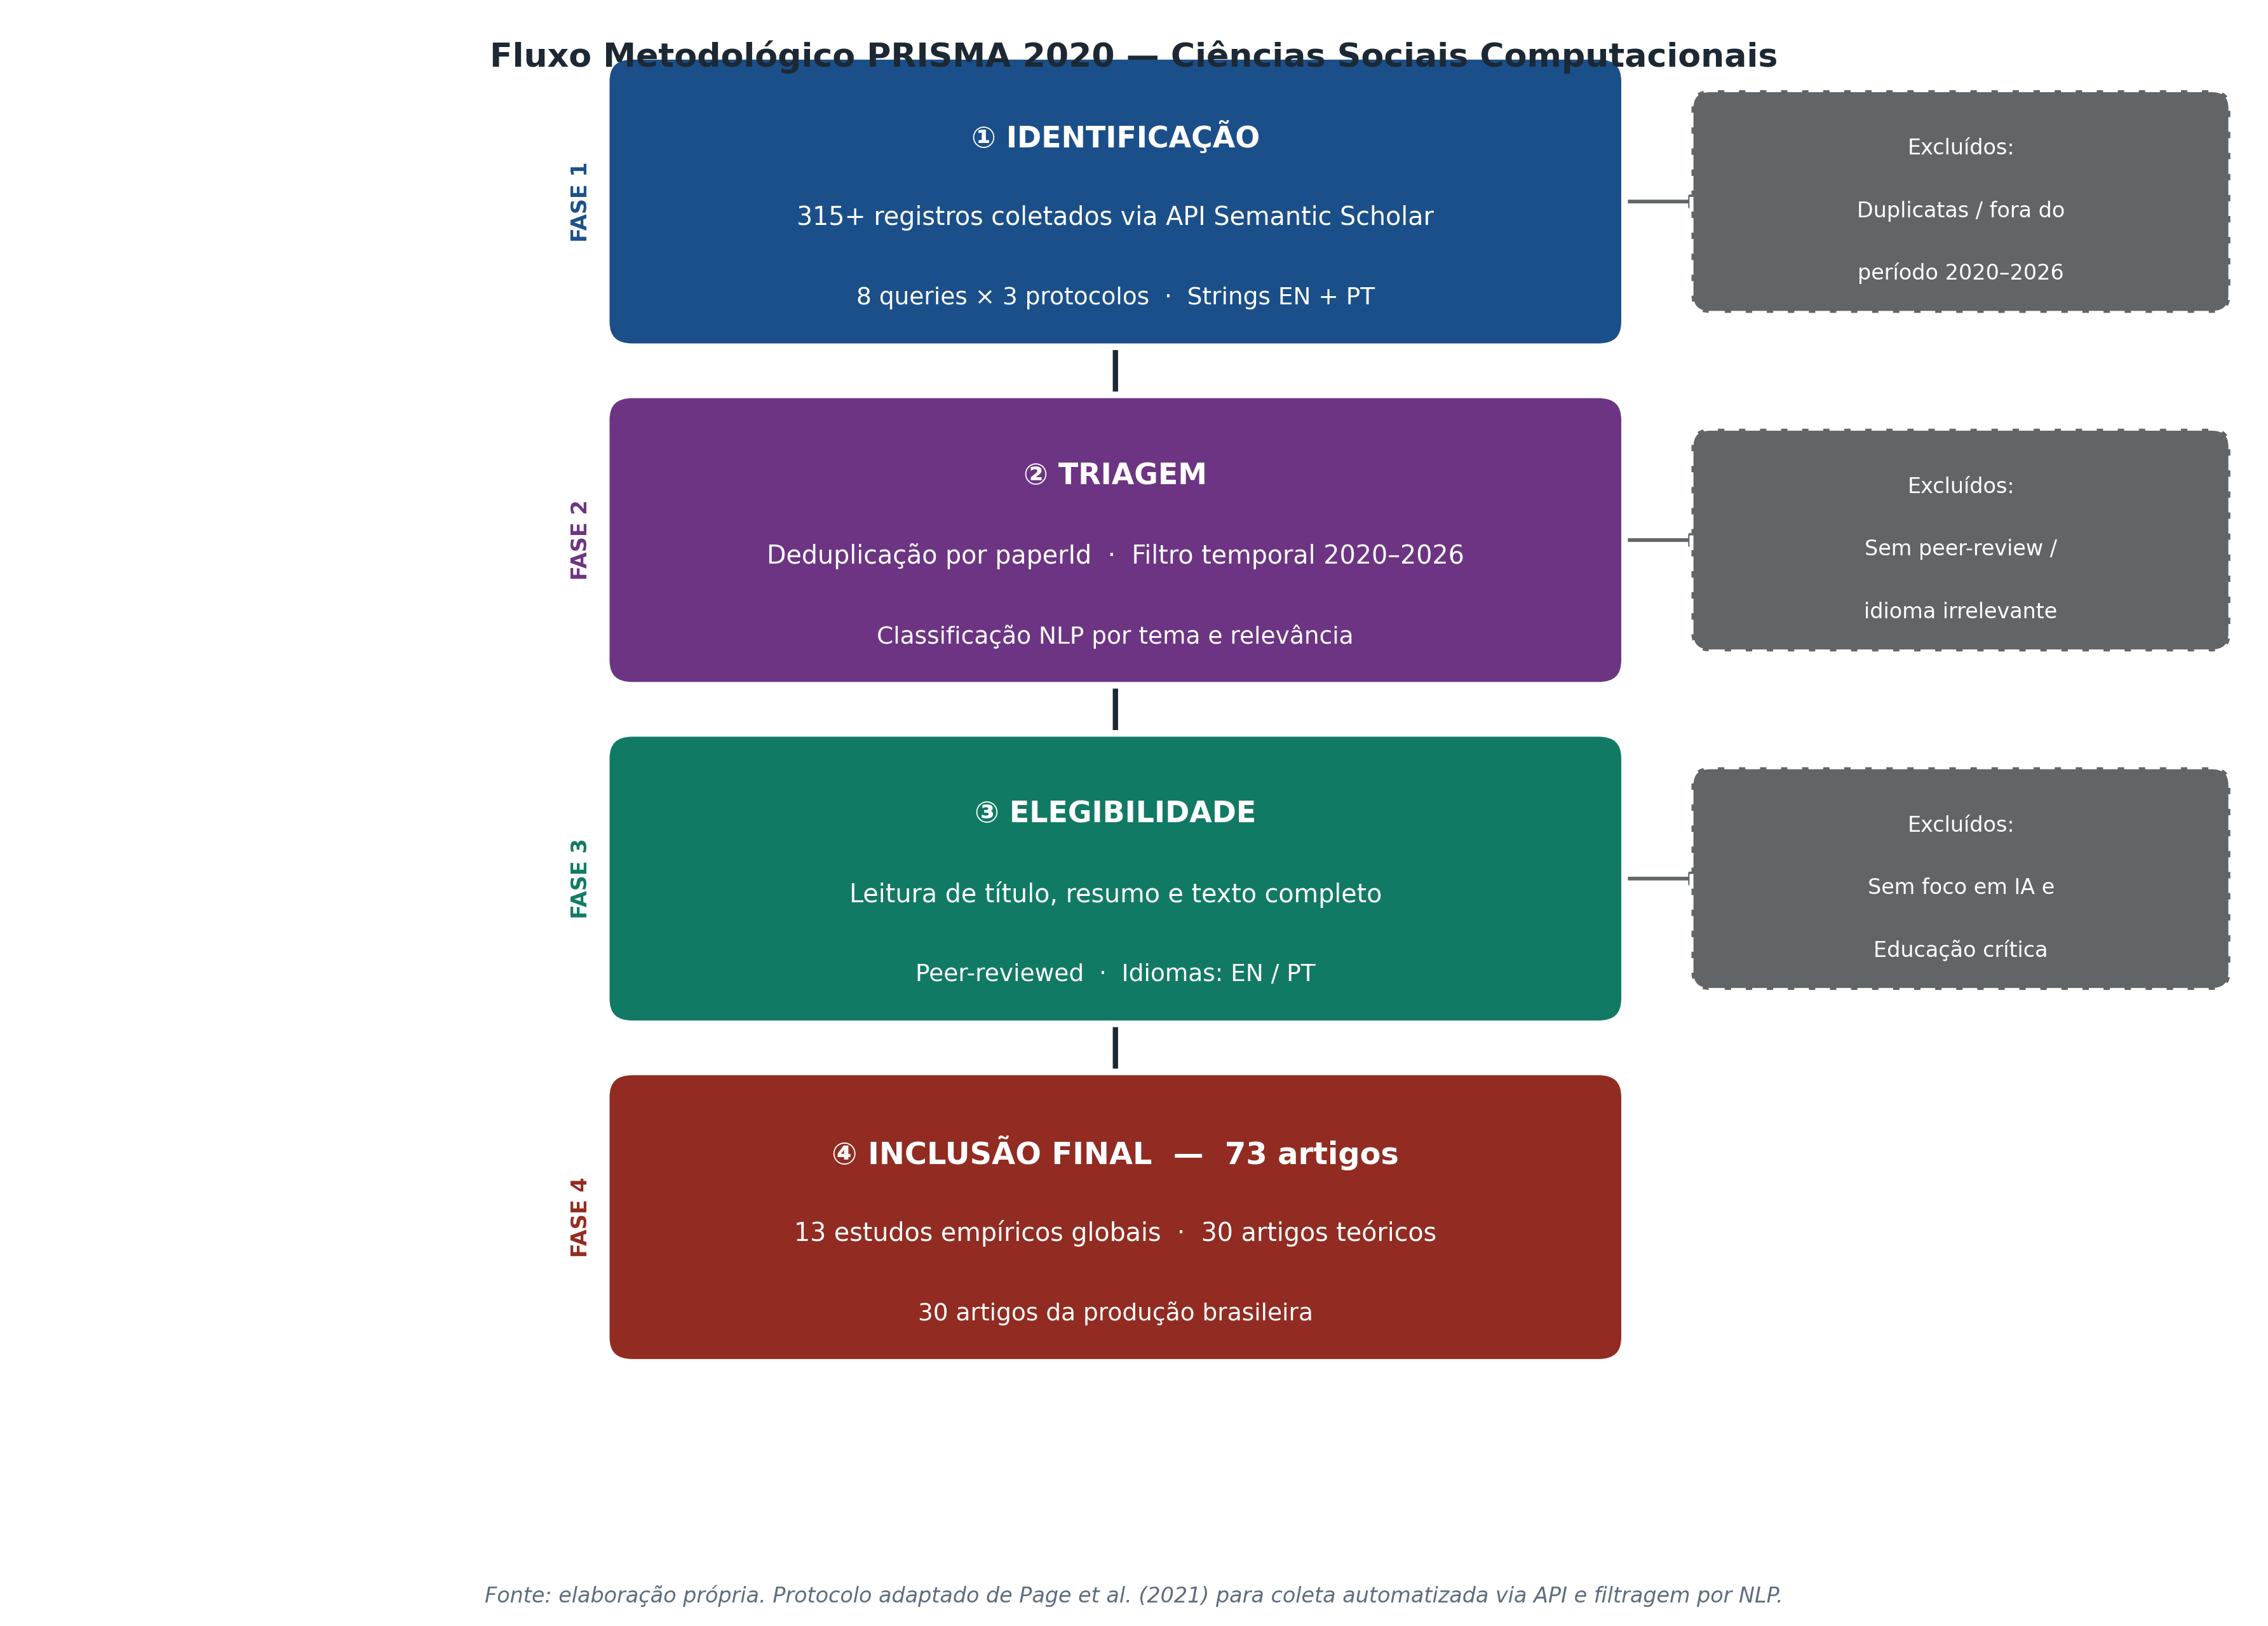
\includegraphics[width=0.90\textwidth]{fig2_prisma_flow.png}
  \caption{Fluxo Metodológico PRISMA~2020 adaptado para Ciências
           Sociais Computacionais.}
  \label{fig:prisma}
\end{figure}

A coleta de dados foi integralmente automatizada mediante a extração via 
\textbf{API oficial do Semantic Scholar} (Graph API v1), garantindo a reprodutibilidade 
exata do corpus ($N{>}315$ registros iniciais). A filtragem e a classificação temática do 
volume de texto valeram-se de técnicas avançadas de Processamento de Linguagem Natural (NLP), 
especificamente \textbf{Topic Modeling} utilizando o algoritmo \textit{Latent Dirichlet Allocation} (LDA). 
O uso de LDA conferiu rigor à identificação de agrupamentos temáticos latentes --- mitigando o 
viés do pesquisador ---, o que permitiu isolar com precisão matemática os discursos de "solucionismo" 
e "iniquidade" dentro do corpus global e nacional.

\begin{figure}[htbp]
  \centering
  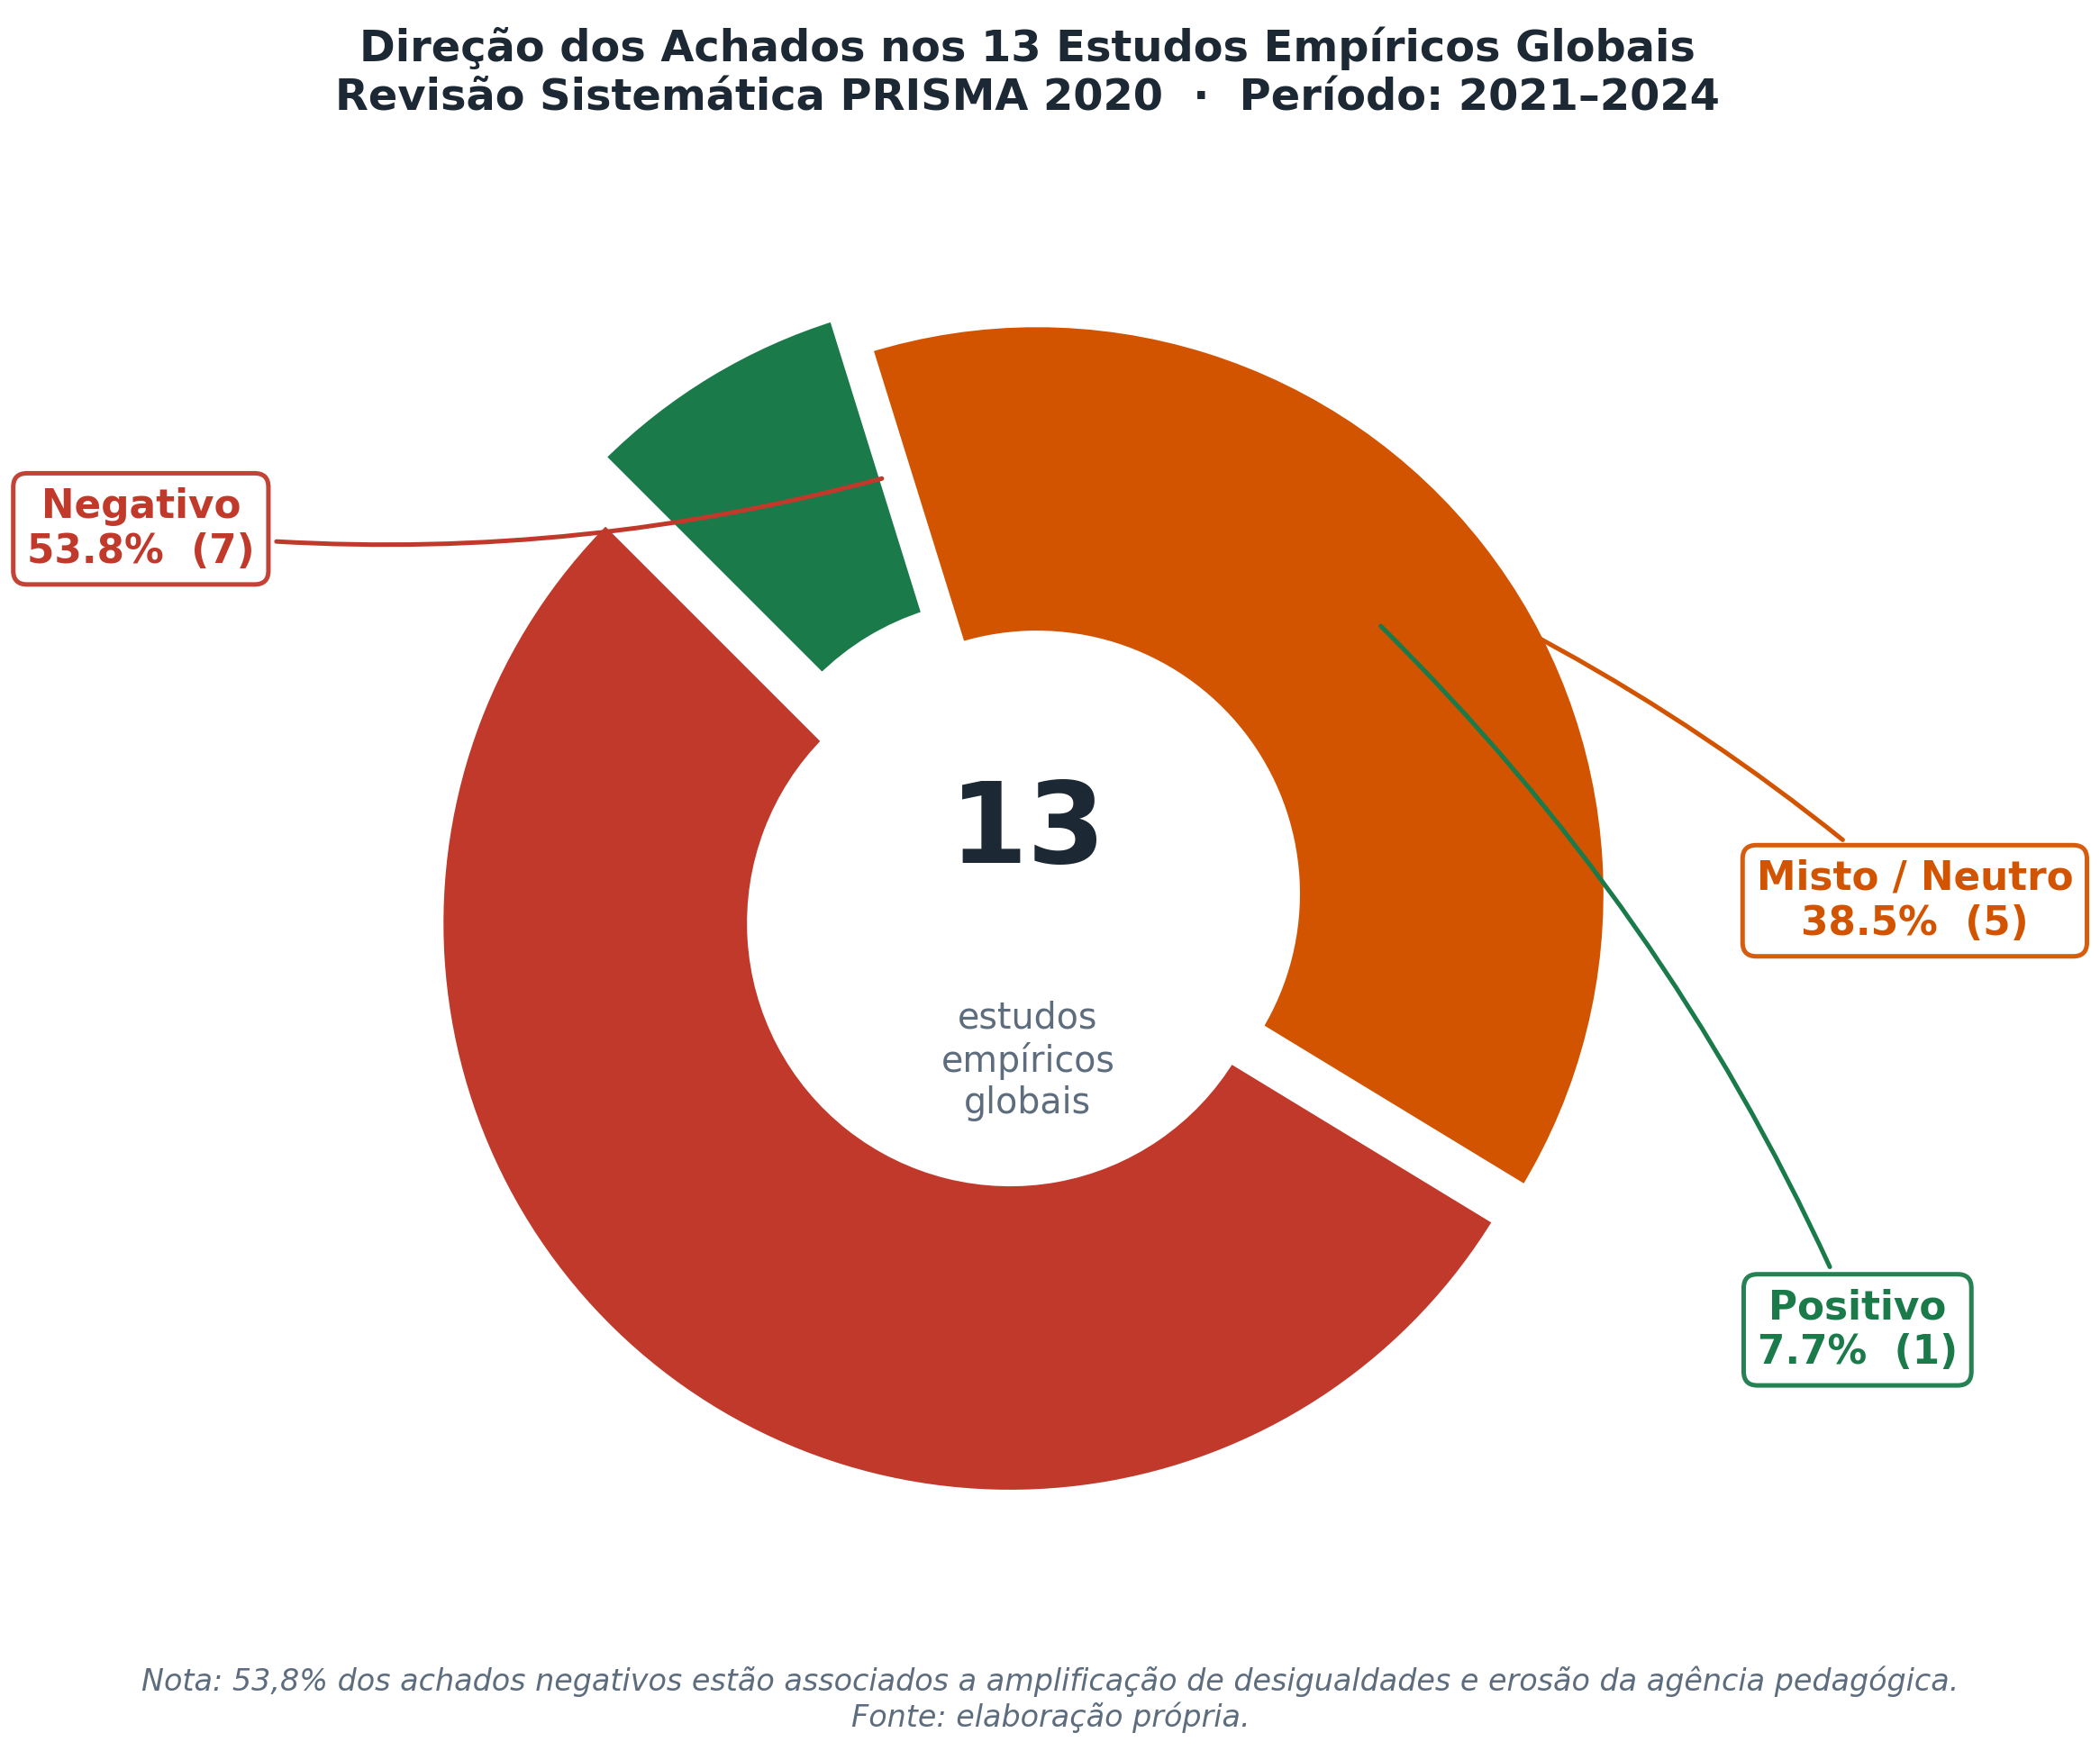
\includegraphics[width=0.68\textwidth]{fig1_empirical_findings.png}
  \caption{Distribuição assimétrica dos achados nos 13 estudos empíricos, evidenciando 53,8\% de resultados negativos.}
  \label{fig:donut}
\end{figure}

% -----------------------------------------------------------
\section{Discussão: O Contexto Brasileiro e a Infraestrutura como Política}
% -----------------------------------------------------------

A integração dos dados oriundos do \textit{brazil\_mapping.csv} evidencia que a questão da 
\textbf{Escola Pública e Desigualdade} (presente em 63,3\% do corpus nacional) não figura como um 
mero apêndice, mas constitui a \textbf{síntese e o cerne argumentativo} deste artigo.

A predominância de vulnerabilidades estruturais documentadas na rede pública brasileira 
articula a transição do nosso ponto de meio para a constatação maior: a infraestrutura é, 
impreterivelmente, política. Quando o currículo, o ritmo de aprendizagem e a avaliação são delegados a 
caixas-pretas algorítmicas --- frequentemente desenvolvidas e hospedadas no Norte Global ---, 
consolida-se uma nova vertente de colonialismo de dados \citep{VanDijck2014, Zuboff2019}. 
Quem detém o controle do código, exerce o poder direto sobre a pedagogia \citep{Noble2018}.

\begin{figure}[htbp]
  \centering
  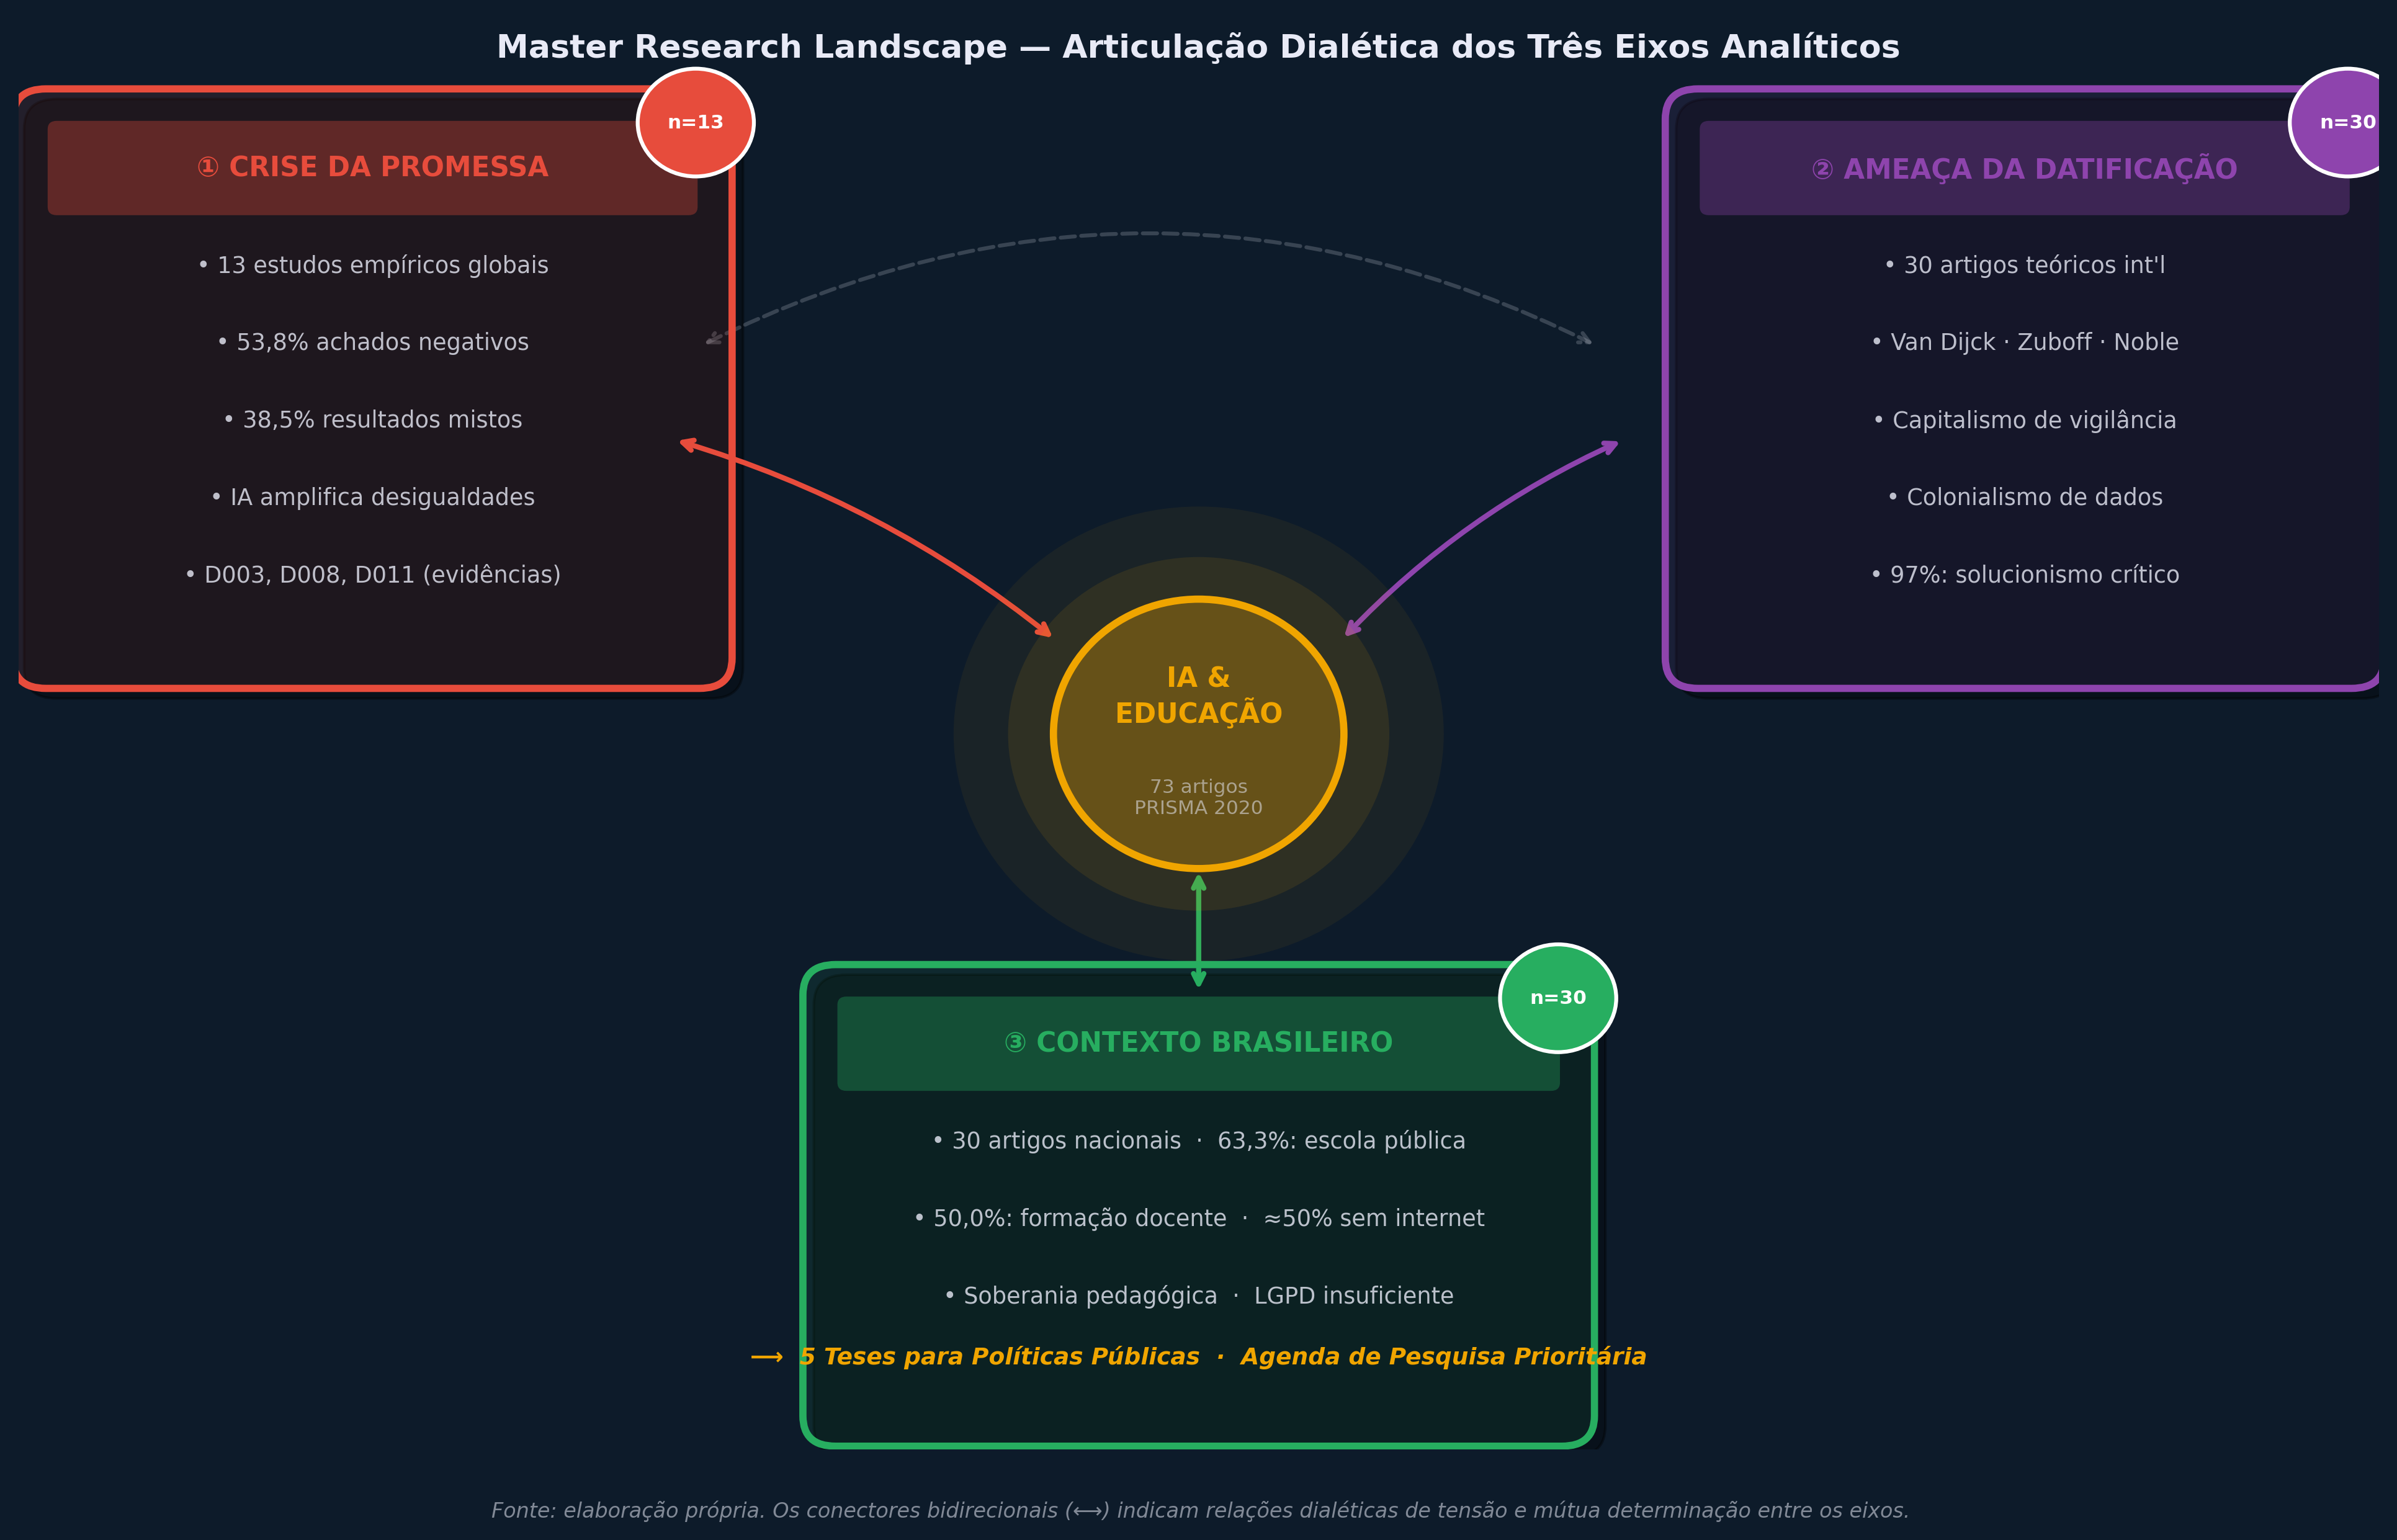
\includegraphics[width=0.95\textwidth]{fig3_dialectical_axes.png}
  \caption{Master Research Landscape: Mapa Conceitual da
           Pesquisa --- Integração Dialética entre Evidências
           Globais, Teoria Crítica e Realidade Brasileira.}
  \label{fig:axes}
\end{figure}

A análise evidencia que a ausência de uma \textbf{infraestrutura digital pública e soberana} 
sujeita as redes estaduais e municipais de ensino à captura corporativa. Os dados coletados das interações 
diárias de milhões de estudantes brasileiros convertem-se em matéria-prima (datificação) para o treinamento 
de modelos de linguagem estrangeiros, perpetuando o ciclo de dependência.

% -----------------------------------------------------------
\section{Conclusão: A Educação como Resistência à Datificação}
% -----------------------------------------------------------

A síntese dos resultados consolida que a IA, em seu formato hegemônico atual, atua primordialmente 
como vetor de assimetria. Contrapor o fetichismo tecnológico requer postular a \textbf{educação como resistência à datificação}.

Evidencia-se a premência de políticas públicas que não se restrinjam à alfabetização digital passiva, 
mas que fomentem a soberania tecnológica. A construção de uma infraestrutura digital pública, transparente 
e auditável é o pré-requisito para que a inteligência artificial sirva à emancipação educacional, 
e não à contínua expropriação de dados das periferias globais.

% -----------------------------------------------------------
\section*{Declaração de Conflito de Interesses}
Os autores declaram ausência de conflito de interesses.

\section*{Financiamento}
A preencher conforme agência financiadora.

\section*{Disponibilidade de Dados e Código}
Repositório: \url{https://github.com/leonardorsl/ia_educacao_research}

% -----------------------------------------------------------
\bibliographystyle{elsarticle-harv}
\bibliography{../references/BIBLIOGRAFIA_MESTRE_IA_EDU}

\end{document}
